\chapter{FPGA Implementation}\label{chap:FPGA_Implementation}
This chapter is devoted to discussing how to implement a Chipyard-generated processor design on a \textbf{local} \gls{fpga} for quicker testing and general use.
Throughout the research project this manual was originally completed in, the Arty \gls{fpga} was used.
An image of the Arty board can be seen in \Cref{fig:Arty_FPGA}.
The Arty board is built using a Xilinx \gls{fpga} module and then Arty creates a board surrounding the particular chip.

\begin{figure}[h!tbp]
  \centering
  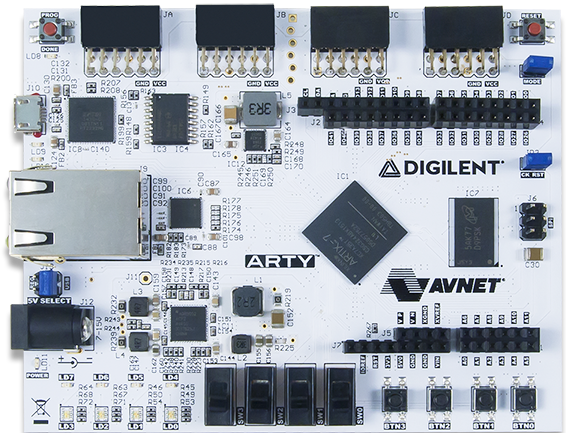
\includegraphics[scale=0.35]{./Arty_FPGA.png}
  \caption{Arty \Gls{fpga}}
  \label{fig:Arty_FPGA}
\end{figure}

\section{About}\label{sec:About}
The Chipyard Framework contains initial support for \gls{fpga} development and simulation of \gls{soc} designs.
At the moment this support is very limited, and is in active development.
As of \today, the best support for \Gls{fpga} Development for the Arty 35T \Gls{fpga} comes from a branch of Chipyard called \href{https://github.com/ucb-bar/chipyard/tree/arty-spi-flash}{arty-spi-flash}.
This branch fixes the \gls{uart} implementation and enables the \gls{spi} flash storage on the Arty \Gls{fpga} to allow users to store programs.

\section{Prerequisites}\label{sec:Prerequisites}
To assist with the proper setup, we approached the \Gls{fpga} implementation of an \Gls{soc} by following the \citetitle{FreedomDevGuide}~\cite{FreedomDevGuide}.
This outlined many of the steps we would eventually need to take, starting with purchasing an \href{https://www.digikey.com/en/products/detail/olimex-ltd/ARM-USB-TINY-H/3471388}{Olimex JTAG Debugger}~\cite{OlimexJTAG}.
Once the final image is flashed to the \Gls{fpga}, the debugger will allow the user to upload C programs and execute them on the RISC-V processor. Without the JTAG Debugger, we were unable to upload programs to the \Gls{fpga}, so this is a necessity.

\begin{figure}[h!tbp]
  \centering
  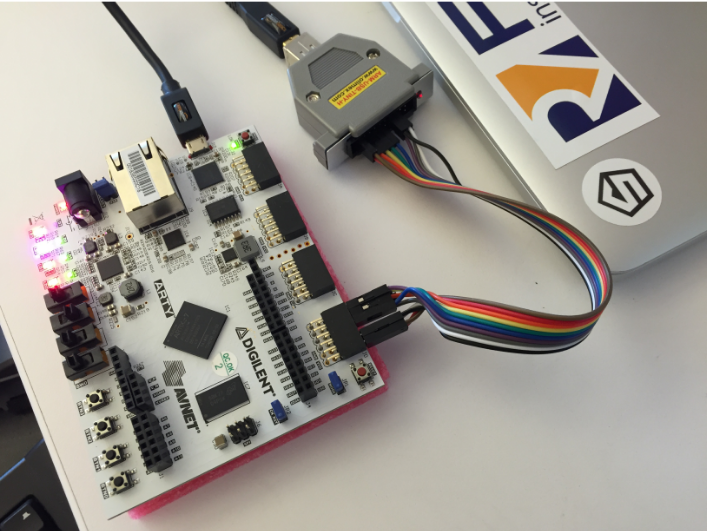
\includegraphics[width=0.7\linewidth]{./OlimexSetup.png}
  \caption{Olimex Debugger Setup~\cite[p.~5]{FreedomDevGuide}}
  \label{fig:olimexsetup}
\end{figure}

\section{Customizing an FPGA Image}\label{sec:Customizing}
In Chipyard, the directory used for all \Gls{fpga} prototyping functionality is \file{chipyard/fpga}, located in the root directory.
Inside this directory there are several important files.

\subsection{Makefile}\label{sec:Customizing_FPGA-Makefile}
Inside the Makefile is where you are able to define a custom subproject as shown in \Cref{subsec:Makefile_SUB_PROJECT}.
This allows users to control what files are compiled and generated for the \Gls{fpga} image.
This is highly recommended as it simplifies the workflow for repeated compilation attempts.

\subsection{Configuration Directory}\label{sec:Customizing_FPGA-Config_Directory}
The configuration directory for the Arty \Gls{fpga} is located under \file{chipyard/fpga/src/main/scala/arty/}.
This directory includes several useful files, including \file{Configs.scala}, \file{HarnessBinders.scala}, \file{IOBinders.scala}, and \file{TestHarness.scala}.

\subsubsection{\file{Configs.scala}}\label{sec:Customizing_FPGA-Configs.scala}
This file is where custom Chipyard SoC configurations are stored and utilized for \Gls{fpga} prototyping. There are several custom configuration parameters for the Arty \Gls{fpga} in this file. The default configuration utilized to make an image for the Arty Board is labeled as "TinyRocketArtyConfig", which then utilized the custom parameters defined for "WithArtyTweaks" and "WithDefaultPeripherals" in the same file. The addresses specified in the "WithDefaultParameters" configurations alter how the memory mapped peripherals for the Arty \Gls{fpga} will be connected.

\subsubsection{\file{HarnessBinders.scala}}\label{sec:Customizing_FPGA-HarnessBinders.scala}
This file is where custom "harness binders" for the Arty \Gls{fpga} are defined. These harness binders utilize pins specified in the master "ArtyShell" pin definitions for the Arty board (provided by Digilent for use in Xilinx Vivado). This file is located under \file{chipyard/fpga/fpga-shells/src/main/scala/shell/xilinx/ArtyShell.scala}. These pin mappings are the same mappings that would be used when interfacing with the Arty board when designing in Xilinx Vivado. Harness binders in this file are provided for the JTAG interface, \Gls{spi} flash, and the \Gls{uart} connector. These three connections are critical to the \Gls{fpga} design, and to ensuring that programs can be successfully uploaded and run on the \Gls{fpga}. It is important to note that the harness binders connects to the "TestHarness", and not the physical IO \cite{Chipyard_IO}. This was done such that separation could be created between the simulation and physical design. To connect to the physical IO pins, IOBinders are also needed.

\subsubsection{\file{IOBinders.scala}}\label{sec:Customizing_FPGA-IOBinders.scala}
This file is where the physical IO pins are connected to the harness binders defined previously. In this file are custom configurations for the \Gls{spi} flash and JTAG connectors that will be utilized in the default design. In the future, additional IOBinders for other peripherals on the Arty \Gls{fpga} should be implemented.

\subsubsection{\file{TestHarness.scala}}\label{sec:Customizing_FPGA-TestHarness.scala}
This file is where miscellaneous connections are made between pins, global clock and reset variable are defined, and the Harness Binders are actually applied to the \Gls{soc} design. No modification to this file shoudl be needed in order to implement new peripheral devices in the future.

\subsection{generated-src Directory}\label{sec:Customizing_FPGA-Generated-src_Directory}

The generated-src directory is the directory in which all files created from compiling the \Gls{soc} design and \Gls{fpga} image will be stored. This means that the memory map, \Gls{fpga} bitstream, and other important files will be stored in this directory. This directory can be found at \file{chipyard/fpga/generated-src}. This directory will not be created until a \Gls{fpga} design run is initiated.



\section{Generating the FPGA Image}\label{sec:Generating_FPGA_Image}
\subsection{Syntax}\label{sec:Generating_FPGA_Image-Syntax}


\section{Using the FPGA Image}\label{sec:Using_FPGA_Image}
\subsection{Flashing the Image}\label{sec:Flash_FPGA_Image}
\subsection{Uploading Programs to the FPGA}\label{sec:Upload_Programs_to_Flashed_FPGA}
%%% Local Variables:
%%% mode: latex
%%% TeX-master: "../doc"
%%% End:
